%%
%% This is file `sample-sigconf.tex',
%% generated with the docstrip utility.
%%
%% The original source files were:
%%
%% samples.dtx  (with options: `sigconf')
%% 
%% IMPORTANT NOTICE:
%% 
%% For the copyright see the source file.
%% 
%% Any modified versions of this file must be renamed
%% with new filenames distinct from sample-sigconf.tex.
%% 
%% For distribution of the original source see the terms
%% for copying and modification in the file samples.dtx.
%% 
%% This generated file may be distributed as long as the
%% original source files, as listed above, are part of the
%% same distribution. (The sources need not necessarily be
%% in the same archive or directory.)
%%
%%
%% Commands for TeXCount
%TC:macro \cite [option:text,text]
%TC:macro \citep [option:text,text]
%TC:macro \citet [option:text,text]
%TC:envir table 0 1
%TC:envir table* 0 1
%TC:envir tabular [ignore] word
%TC:envir displaymath 0 word
%TC:envir math 0 word
%TC:envir comment 0 0
%%
%%
%% The first command in your LaTeX source must be the \documentclass
%% command.
%%
%% For submission and review of your manuscript please change the
%% command to \documentclass[manuscript, screen, review]{acmart}.
%%
%% When submitting camera ready or to TAPS, please change the command
%% to \documentclass[sigconf]{acmart} or whichever template is required
%% for your publication.
%%
%%



\documentclass[sigconf]{acmart}

\usepackage{subfig}

%%
%% \BibTeX command to typeset BibTeX logo in the docs
\AtBeginDocument{%
  \providecommand\BibTeX{{%
    Bib\TeX}}}

%% Rights management information.  This information is sent to you
%% when you complete the rights form.  These commands have SAMPLE
%% values in them; it is your responsibility as an author to replace
%% the commands and values with those provided to you when you
%% complete the rights form.
\setcopyright{acmcopyright}
\copyrightyear{2023}
\acmYear{2023}
\acmDOI{XXXXXXX.XXXXXXX}

%% These commands are for a PROCEEDINGS abstract or paper.
% \acmConference[Conference acronym 'XX]{Make sure to enter the correct
%   conference title from your rights confirmation emai}{June 03--05,
%   2018}{Woodstock, NY}
%%
%%  Uncomment \acmBooktitle if the title of the proceedings is different
%%  from ``Proceedings of ...''!
%%
%%\acmBooktitle{Woodstock '18: ACM Symposium on Neural Gaze Detection,
%%  June 03--05, 2018, Woodstock, NY}
% \acmPrice{15.00}
% \acmISBN{978-1-4503-XXXX-X/18/06}


%%
%% Submission ID.
%% Use this when submitting an article to a sponsored event. You'll
%% receive a unique submission ID from the organizers
%% of the event, and this ID should be used as the parameter to this command.
\acmSubmissionID{123-A56-BU3}

%%
%% For managing citations, it is recommended to use bibliography
%% files in BibTeX format.
%%
%% You can then either use BibTeX with the ACM-Reference-Format style,
%% or BibLaTeX with the acmnumeric or acmauthoryear sytles, that include
%% support for advanced citation of software artefact from the
%% biblatex-software package, also separately available on CTAN.
%%
%% Look at the sample-*-biblatex.tex files for templates showcasing
%% the biblatex styles. 
%%

%%
%% The majority of ACM publications use numbered citations and
%% references.  The command \citestyle{authoryear} switches to the
%% "author year" style.
%%
%% If you are preparing content for an event
%% sponsored by ACM SIGGRAPH, you must use the "author year" style of
%% citations and references.
%% Uncommenting
%% the next command will enable that style.
%%\citestyle{acmauthoryear}


%%
%% end of the preamble, start of the body of the document source.
\begin{document}

%%
%% The "title" command has an optional parameter,
%% allowing the author to define a "short title" to be used in page headers.
\title{Performance Evaluation of 6DoF Localization on Mobile Devices}

%%
%% The "author" command and its associated commands are used to define
%% the authors and their affiliations.
%% Of note is the shared affiliation of the first two authors, and the
%% "authornote" and "authornotemark" commands
%% used to denote shared contribution to the research.
\author{Chandra Kiran Viswanath Balusu}
% \authornote{Both authors contributed equally to this research.}
\email{cbalusu@gmu.edu}
% \orcid{1234-5678-9012}
% \authornotemark[1]
\affiliation{%
  \institution{George Mason University}
  \streetaddress{4400 University Dr}
  \city{Fairfax}
  \state{Virginia}
  \country{USA}
  \postcode{22030}
}

\author{Bharath Chandra Nimmala}
% \authornotemark[2]
\email{bnimmala@gmu.edu}
\affiliation{%
  \institution{George Mason University}
  \streetaddress{4400 University Dr}
  \city{Fairfax}
  \state{Virginia}
  \country{USA}
  \postcode{22030}
}

%%
%% By default, the full list of authors will be used in the page
%% headers. Often, this list is too long, and will overlap
%% other information printed in the page headers. This command allows
%% the author to define a more concise list
%% of authors' names for this purpose.
% \renewcommand{\shortauthors}{Trovato et al.}

%%
%% The abstract is a short summary of the work to be presented in the
%% article.
\begin{abstract}
The rapid advancement of mobile device technology has driven the need for accurate and efficient localization in three-dimensional (3D) space. Six Degrees of Freedom (6DoF) localization is a promising technology that addresses this challenge by providing precise position and orientation information. In this research project, we aim to evaluate the performance of 6DoF localization on mobile devices such as accuracy and latency. The evaluation of 6DoF (six degrees of freedom) localization on mobile devices is crucial for improving the accuracy and reliability of localization algorithms, which can lead to the development of more effective techniques for 3D space localization. This assessment is particularly important for applications that require precise and dependable localization, ensuring their feasibility and effectiveness. Advancements in this research area can have significant implications for computer vision, robotics, and spatial computing, expanding researcher's understanding of how to enable 3D sensing and spatial awareness in various mobile device applications and settings.
\end{abstract}

%%
%% The code below is generated by the tool at http://dl.acm.org/ccs.cfm.
%% Please copy and paste the code instead of the example below.
%%
% \begin{CCSXML}
% <ccs2012>
%  <concept>
%   <concept_id>10010520.10010553.10010562</concept_id>
%   <concept_desc>Computer systems organization~Embedded systems</concept_desc>
%   <concept_significance>500</concept_significance>
%  </concept>
%  <concept>
%   <concept_id>10010520.10010575.10010755</concept_id>
%   <concept_desc>Computer systems organization~Redundancy</concept_desc>
%   <concept_significance>300</concept_significance>
%  </concept>
%  <concept>
%   <concept_id>10010520.10010553.10010554</concept_id>
%   <concept_desc>Computer systems organization~Robotics</concept_desc>
%   <concept_significance>100</concept_significance>
%  </concept>
%  <concept>
%   <concept_id>10003033.10003083.10003095</concept_id>
%   <concept_desc>Networks~Network reliability</concept_desc>
%   <concept_significance>100</concept_significance>
%  </concept>
% </ccs2012>
% \end{CCSXML}

% \ccsdesc[500]{Computer systems organization~Embedded systems}
% \ccsdesc[300]{Computer systems organization~Redundancy}
% \ccsdesc{Computer systems organization~Robotics}
% \ccsdesc[100]{Networks~Network reliability}

%%
%% Keywords. The author(s) should pick words that accurately describe
%% the work being presented. Separate the keywords with commas.
\keywords{6DoF localization, Performance Evaluation, COLMAP, Structure-from-Motion(SfM)}
%% A "teaser" image appears between the author and affiliation
%% information and the body of the document, and typically spans the
%% page.
% \begin{teaserfigure}
%   \includegraphics[width=\textwidth]{sampleteaser}
%   \caption{Seattle Mariners at Spring Training, 2010.}
%   \Description{Enjoying the baseball game from the third-base
%   seats. Ichiro Suzuki preparing to bat.}
%   \label{fig:teaser}
% \end{teaserfigure}

% \received{20 February 2007}
% \received[revised]{12 March 2009}
% \received[accepted]{5 June 2009}

%%
%% This command processes the author and affiliation and title
%% information and builds the first part of the formatted document.
\maketitle

\section{Introduction}

\subsection{Statement of the Problem, Significance, and Goals}
6DoF localization is a technology that enables the identification of an object's position and orientation in three-dimensional space, offering six degrees of freedom, which comprise three for translation and three for rotation. This technology finds applications in diverse fields, such as robotics, virtual reality, and mobile device tracking. 6DoF localization enables robots to navigate more precisely, enhances the immersive experience in virtual reality, and improves location tracking and augmented reality on mobile devices. Evaluating the performance of 6DoF localization\cite{benchmarking6dof} on mobile devices involves assessing its accuracy, speed, and reliability. To achieve this, various metrics can be utilized. Some of the metrics used for evaluating the performance of 6DoF localization on mobile devices include Localization accuracy, Latency, Robustness, Power consumption, etc., 


The assessment of 6DoF localization on mobile devices is significant as it has the potential to enhance the precision and dependability of localization algorithms\cite{6DOFfuturework} and lead to the creation of more effective techniques for localizing in 3D space. This evaluation is essential for various applications that demand accurate and dependable localization, ensuring that these applications are feasible and effective. Progress in this research area can have far-reaching consequences for fields like computer vision, robotics, and spatial computing, deepening the researcher’s comprehension of how to enable 3D sensing and spatial awareness in different mobile device applications and environments.


\subsection{Background}
A significant amount of research was conducted on 6DoF Localization on mobile devices, especially related to performance evaluation\cite{benchmarking6dof} . For example, A study conducted in 2016, "Real-time 6DoF Tracking for Mobile Augmented Reality"\cite{6doftrackingmobilear}, introduced a 6DoF tracking system for mobile augmented reality applications, which was evaluated based on its tracking accuracy, latency, and power consumption. Results from the evaluation indicated that the proposed system is appropriate for real-time applications as it offers the necessary tracking accuracy and low latency, with minimal power consumption. Another study conducted in 2017, 6DoF Object Tracking based on 3D Scans for Augmented Reality Remote Live Support”\cite{6dof2017}, assessed the performance of various 6DoF tracking techniques that could be employed for mobile augmented reality applications. The focus was on comparing feature-based and model-based techniques and evaluating their accuracy, robustness, and computational efficiency.


Evaluating the performance of 6DoF localization\cite{benchmarking6dof} on mobile devices involves several methods, and researchers have used different techniques for this purpose. Accuracy of localization is a primary focus, but other factors such as latency, robustness, and power consumption are also evaluated. Evaluation methods can be either quantitative, involving measures like mean error, precision, and recall, or qualitative, relying on user feedback and subjective evaluations. With the advancement of sensors and processing power in mobile devices, the performance of 6DoF localization\cite{benchmarking6dof} on such devices is predicted to improve. Future research on 6DoF localization\cite{6DOFfuturework} is likely to concentrate on developing more precise and dependable algorithms, along with integrating multiple techniques and sensors to improve the technology's performance. Additionally, efforts may be made to design systems that consume less energy and increase the technology's ability to operate in different environments.

\section{Software's Used}
\begin{itemize}
\item{\textbf{COLMAP\cite{schoenberger2016sfm}: }
COLMAP is a computer vision software package for 3D reconstruction and image-based localization, developed by Johannes L. Schönberger and Jan-Michael Frahm. It can be used for a variety of applications, including robotics, augmented reality, and virtual reality. The software takes a set of 2D images as input and produces a 3D point cloud and a textured mesh as output. It uses feature detection and matching techniques to find correspondences between images, and then estimates the camera poses and the 3D structure of the scene using geometric and photometric constraints. COLMAP supports a wide range of camera models, including pinhole, fisheye, and panoramic cameras, and can handle large datasets with hundreds of thousands of images. It also provides tools for filtering and refining the reconstruction, as well as for exporting the results to other software packages.} 

\item{\textbf{PyCOLMAP: }
PyCOLMAP is a Python package that provides a Python interface for COLMAP, a popular open-source software for computer vision that allows you to perform 3D reconstruction from images. With PyCOLMAP, you can use the COLMAP algorithms from within Python, which allows you to automate and customize the 3D reconstruction process.}

\item{\textbf{Hloc\cite{hlocatlargescale}: }
Hierarchical localization is a technique used in computer vision and robotics to locate an agent (e.g., a robot or a person) in an environment using a pre-built map. The environment is divided into multiple levels of increasing granularity, which reduces the search space and increases accuracy. Building the map involves constructing a 3D model of the environment using sensors, which is divided into levels. Localizing the agent involves matching sensory data with the map at the coarsest level first and refining the estimate at finer levels. Hierarchical localization has applications in various fields, enabling accurate and efficient localization in complex and dynamic environments.}

\item{\textbf{FastAPI: }
FastAPI is a web framework for building APIs in Python 3.7+ that is fast, modern, and easy to use. It uses asynchronous programming to handle multiple requests at once, and provides built-in support for OpenAPI and JSON Schema for automatic API documentation and testing. FastAPI is intuitive and easy to learn, supporting standard HTTP methods and features like dependency injection, background tasks, and security measures like OAuth2 and JWT tokens. FastAPI is gaining popularity for its high performance and modern features.}
\item{\textbf{aiofiles: }
aiofiles is a Python library that allows developers to work with files asynchronously, providing a simple API for opening, closing, reading, and writing files, as well as working with file descriptors. It enables file operations to be performed without blocking the event loop, making it useful for applications with multiple simultaneous file operations, such as web applications. aiofiles supports binary and text modes and provides functions for working with file paths and directories. It integrates well with asyncio libraries and frameworks and can improve the performance and efficiency of applications that rely on file I/O operations.}
\item{\textbf{aiopath: }
aiopath is a Python library that offers an asynchronous interface for path-related operations in file systems. It has a simple API that is similar to the standard os.path API, with functions for joining, splitting, and normalizing paths, and working with file and directory names. It enables path-related operations to be performed asynchronously, making it beneficial for web applications that need to access file system paths simultaneously. aiopath also supports paths that point to remote file systems and can integrate well with other asyncio libraries and frameworks. Overall, aiopath can enhance the performance and efficiency of path-related operations in asynchronous Python applications.}
\item{\textbf{uvicorn: }
Uvicorn is an asynchronous web server for Python designed to handle high-concurrency HTTP requests and other protocols. It is built on top of the asyncio library and is capable of handling thousands of requests per second with low latency and resource usage. Uvicorn supports features like WebSockets, HTTP/2, and UNIX sockets, and works with other ASGI-compatible frameworks such as FastAPI, Starlette, and Quart. It is easy to use and configure, providing a simple command-line interface and support for configuration via environment variables, command-line options, and configuration files.}
\item{\textbf{Unity Engine\cite{unityengine}: }
The Unity Engine is a cross-platform game engine widely used for developing video games, simulations, and interactive applications. It supports 2D and 3D graphics with a range of tools for creating and manipulating 3D models, textures, and animations, as well as scripting using C\#. Unity provides a powerful editor, libraries, plugins, and third-party extensions. It also supports collaboration and version control for teams working on large-scale projects. Unity's accessibility and versatility have made it popular among indie developers and large game development studios alike.}

\end{itemize}


\section{Preliminary Testing}
We have conducted our initial testing using the dataset which contains 1273 high-resolution images of the interior and exterior of “Graham” memorial hall at UNC Chapel Hill and generated the spatial map of the hall using COLMAP. The generated map has 407114 points in the point cloud. The generated map can be found in \textbf{Figure \ref{fig:graham}} in page \pageref{fig:graham}.

\begin{figure}%
    \centering
    \subfloat[\centering]{{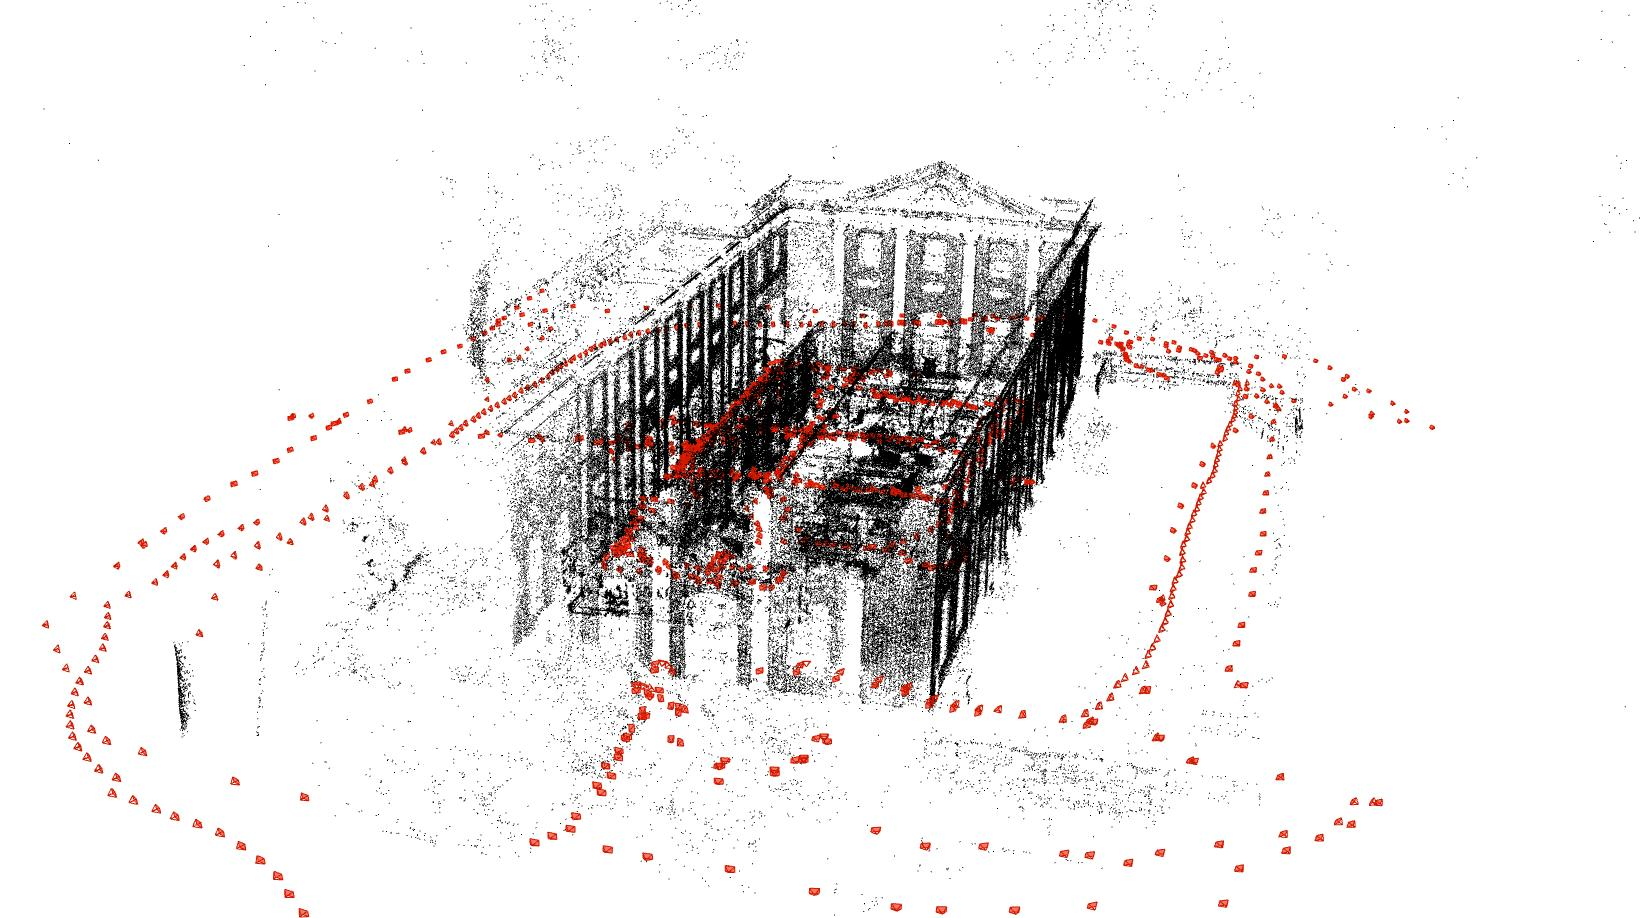
\includegraphics[width=\linewidth]{images/graham/1.jpg} }}%
    \qquad
    \subfloat[\centering]{{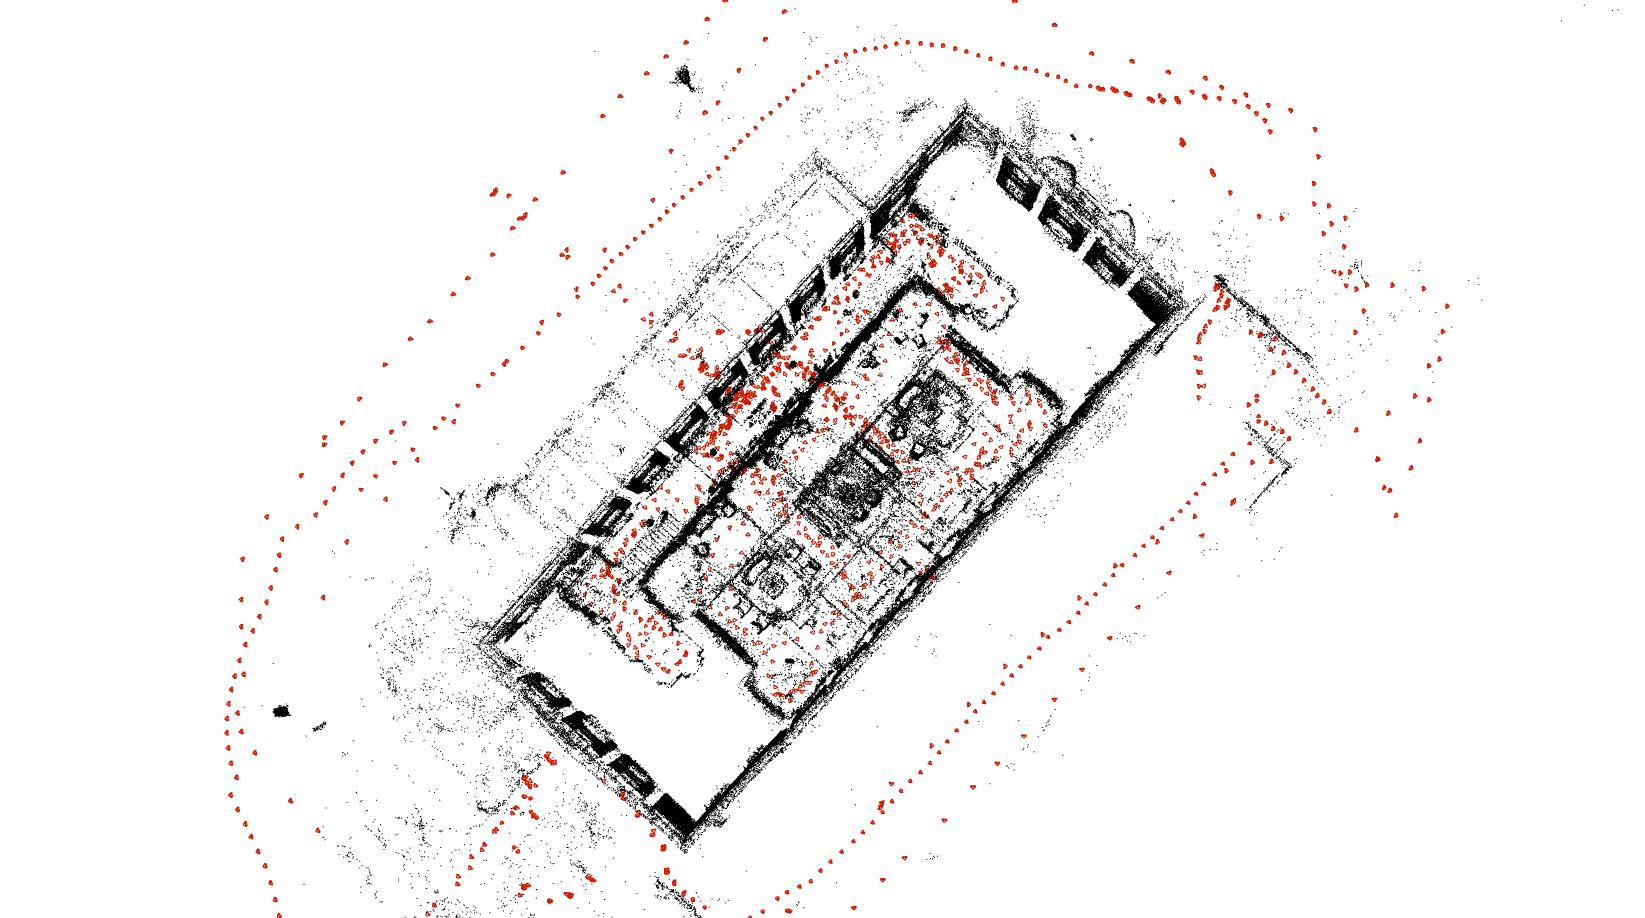
\includegraphics[width=\linewidth]{images/graham/2.jpg} }}%
    \qquad
    \subfloat[\centering]{{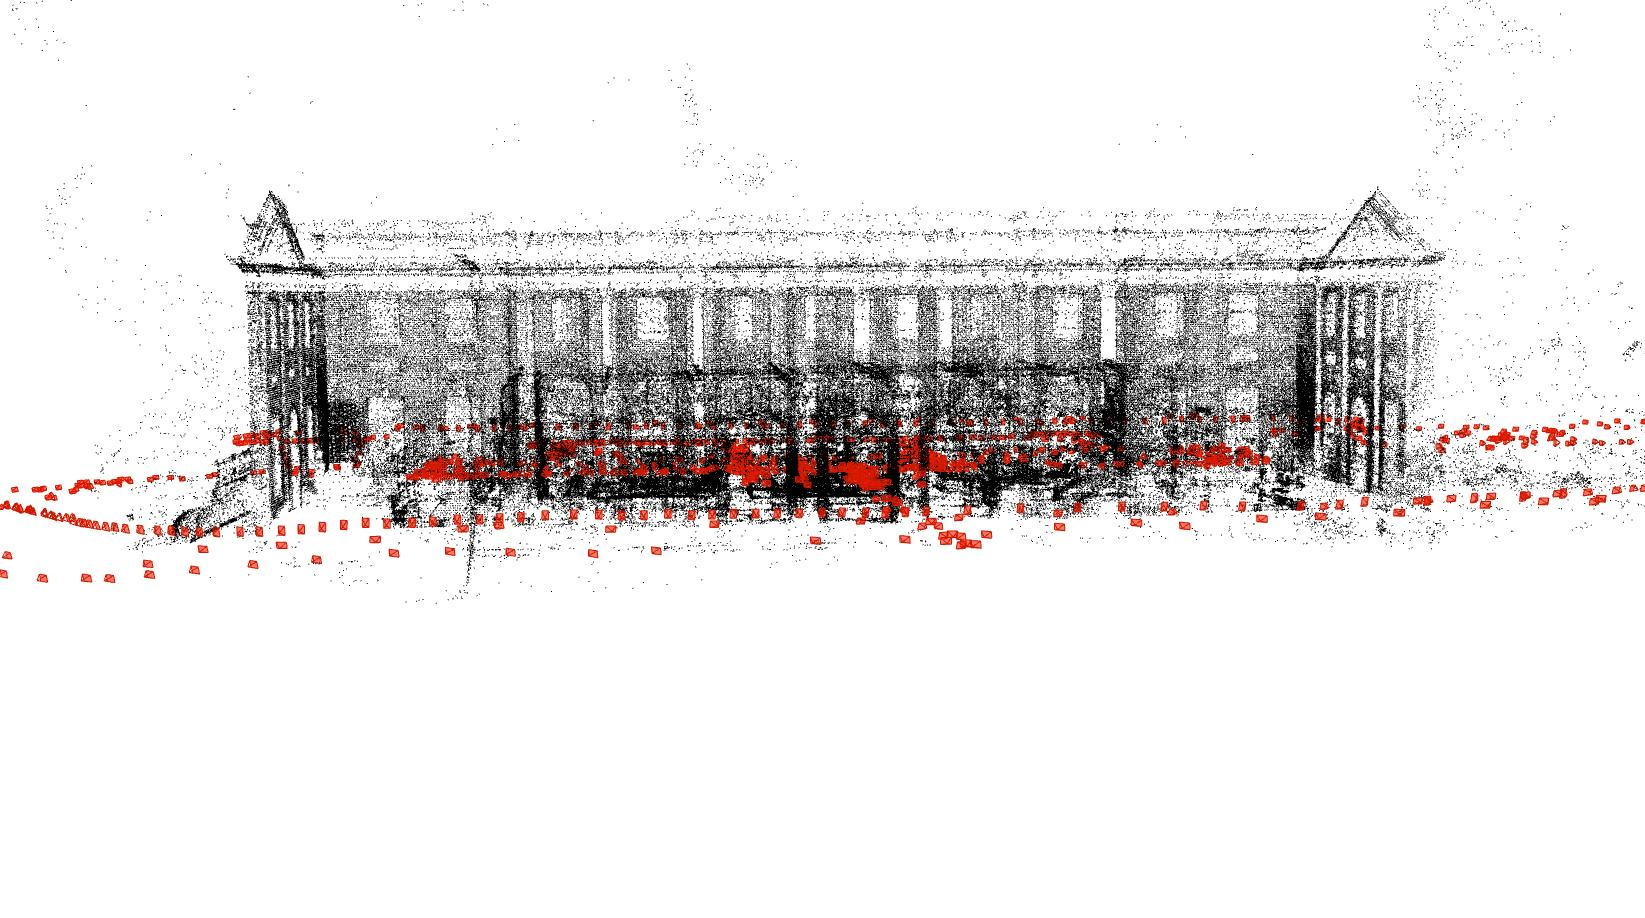
\includegraphics[width=\linewidth]{images/graham/3.jpg} }}%
    \caption{Spatial Map generated from the dataset of Graham Hall.}
    \label{fig:graham}%
\end{figure}

\section{Dataset Collection}
We have captured 279 aerial images of the George Mason University Field House located at 4501 University Dr, Fairfax, VA 22030 using DJI mini 2 drone.


\section{Methodology}
In order to evaluate the performance of 6DoF localization using Hloc\cite{hloc} on mobile devices, we need a client-server REST API architecture as compared to mobile devices because of the computing power constraint. 
\newline 
\newline 
The design of the REST API server is as follows:
\begin{itemize}
\item{The REST API server is based on FAST API framework which is written in Python programming language that leverages asyncio concurrency module that increases the speed of the application.}
\item{As we are using Hloc package written in Python, we extended it from the source code by creating a Git submodule in the Git repository.}
\item{In order to facilitate multiple datasets and outputs, the REST API is designed to handle multiple sessions that uses UUID\cite{uuid} which are stored in the underlying SQLite3\cite{SQLite3} to differentiate sessions.The end points can be seen in the \textbf{Figure \ref{fig:restsession}}
\begin{figure}[h]
  \centering
  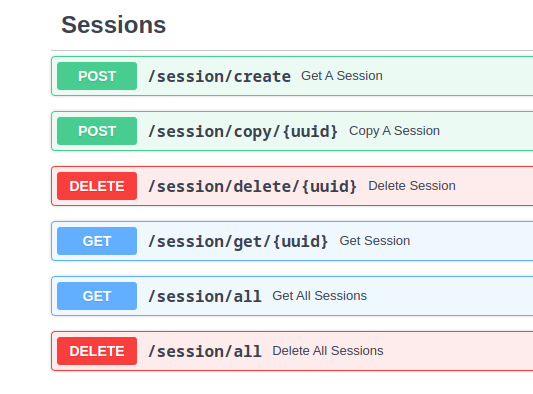
\includegraphics[width=5cm]{images/restapi/1.png}
  \caption{REST API Session Handling Endpoints}
  \label{fig:restsession}
\end{figure}
}

\item{To ensure security to the designed REST API, we require apikey to make calls to the API.}
\item{To upload the dataset, we have an endpoint and there is another endpoint to upload the SfM generated in COLMAP. The end points can be seen in the \textbf{Figure \ref{fig:restdataset}}
\begin{figure}[h]
  \centering
  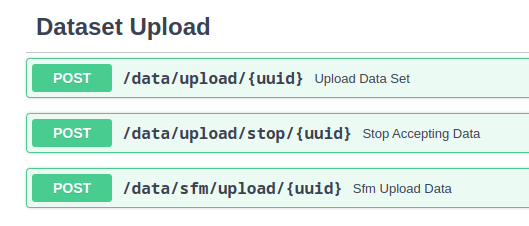
\includegraphics[width=5cm]{images/restapi/2.png}
  \caption{Dataset and SfM Upload Endpoints}
  \label{fig:restdataset}
\end{figure}
}
\item{For feature extraction and mapping, we designed two endpoints where feature extraction and matching uses one endpoint and map generation uses another endpoint. The end points can be seen in the \textbf{Figure \ref{fig:restpipeline}}
\begin{figure}[h]
  \centering
  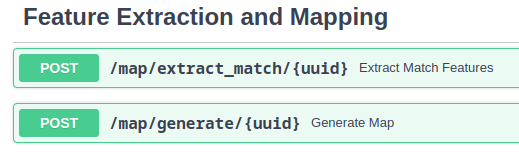
\includegraphics[width=5cm]{images/restapi/3.png}
  \caption{Feature Extraction, Matching and Mapping}
  \label{fig:restpipeline}
\end{figure}
}
\item{For the Localization of the Query images, there is one endpoint which returns the pose estimations after the localization and the Latency.}
\item{There are few more endpoints that streams the Point cloud to the client which are in the Development phase.}
\end{itemize}

We are using the source code of localization unity application developed by Yiyang Shi, which was provided to us by Nan Wu. We are currently modifying some of our endpoints to work with this application seamlessly. 

\section{Results achieved to date}
Using the dataset of the GMU field house which we collected, we ran the SfM pipeline multiple times with different configurations in order to achieve the best results. The results are as follows:

\subsection{Spatial Maps Generated Using Different Configurations}
The below shown figures are spatial maps that were generated using different configurations. The configurations are mentioned in the figure captions.

\textbf{Configuration 1: }
\textit{The below two figures belong to SfM, generated using SuperPoint Aachen for Extraction and SuperGlue Neural Net for Matching with SfM pairs from NETVLAD Global Feature Extractor.}

\begin{figure}[H]%
    \centering
    \subfloat[\centering]{{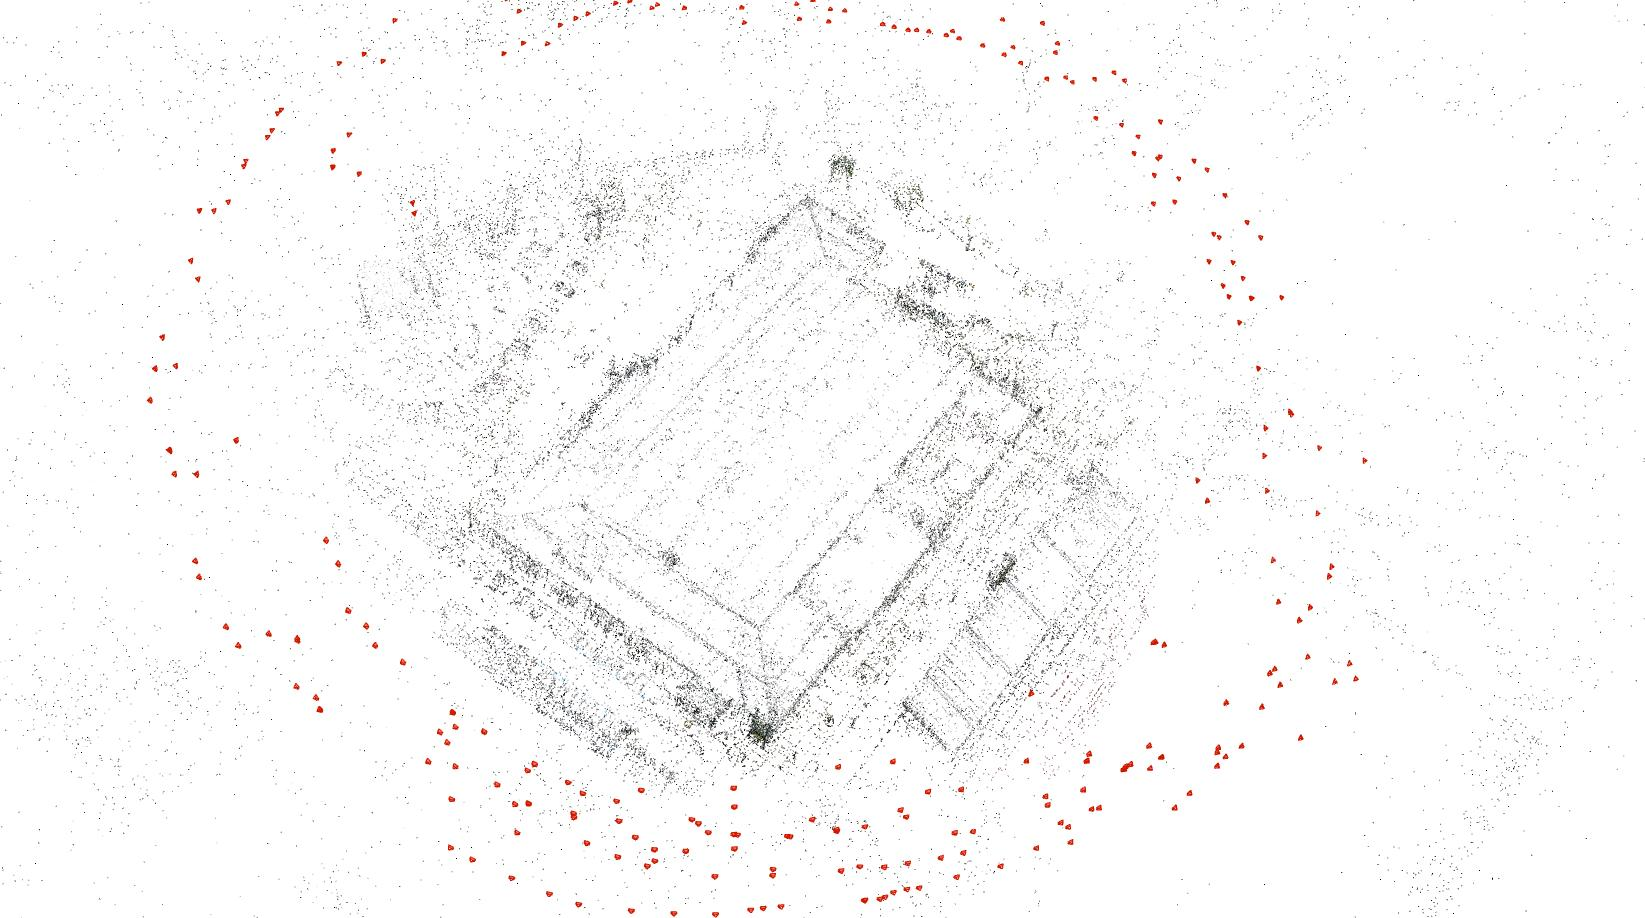
\includegraphics[width=\linewidth]{images/results/sp_sg_global_fts.jpg} }}%
    \qquad
    \subfloat[\centering]{{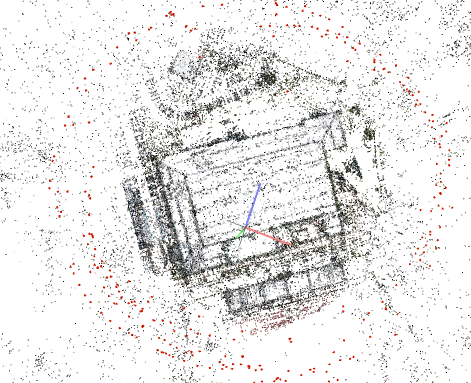
\includegraphics[width=\linewidth]{images/results/spsg_netvlad.png} }}%
    \caption{Point Cloud of the Reconstruction with 96971 Points}
    \label{fig:SPSGGE}%
\end{figure}

\textbf{Configuration 2: }
\textit{The below figure belong to SfM, generated using Sift Extraction with 16384 maximum features from each image and Exhaustive Matching within the COLMAP.}

\begin{figure}[H]
  \centering
  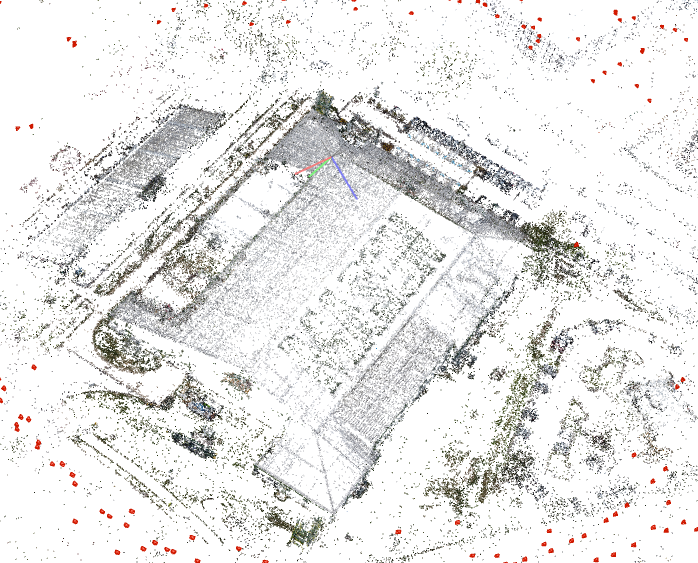
\includegraphics[width=\linewidth]{images/results/sfm_sift_16384.png}
  \caption{Point Cloud of the Reconstruction with 167275 Points}
  \label{fig:sift_basic}
\end{figure}

\textbf{Configuration 2: }
\textit{The below figure belong to SfM, generated using Sift Extraction with 24576 maximum features and Exhaustive Matching within the COLMAP.}

\begin{figure}[H]
  \centering
  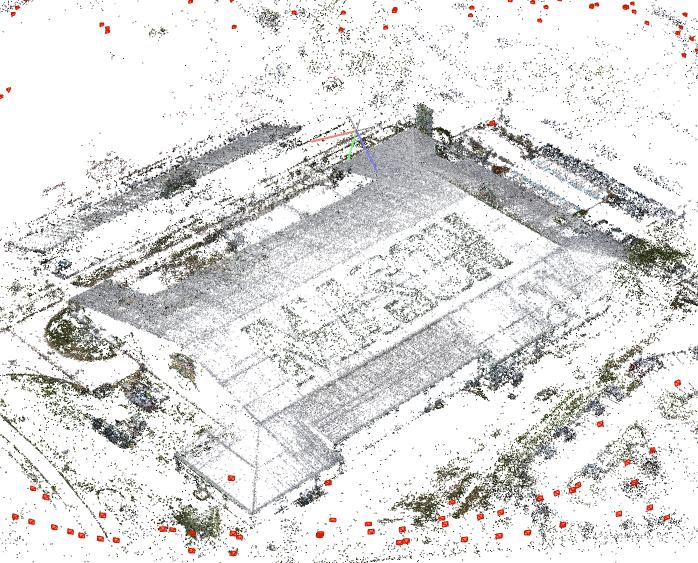
\includegraphics[width=\linewidth]{images/results/sfm_sift_24576.png}
  \caption{Point Cloud of the Reconstruction with 307829 Points}
  \label{fig:sift_more}
\end{figure}


From the above three cases we can say that SIFT is more robust when compared to Superpoint Extraction and moreover when the number of features that are being extracted increases, we were able to see a more dense point cloud each time. SIFT Extraction and Matching took less time compared to different configurations.
\\ Now that we have a sparse SfM with cameras that have intrinsic values, we then proceeded with the Dense Reconstruction.

The Dense Reconstruction that we generated has 42207561 colored points
\begin{figure}[H]%
    \centering
    \subfloat[\centering]{{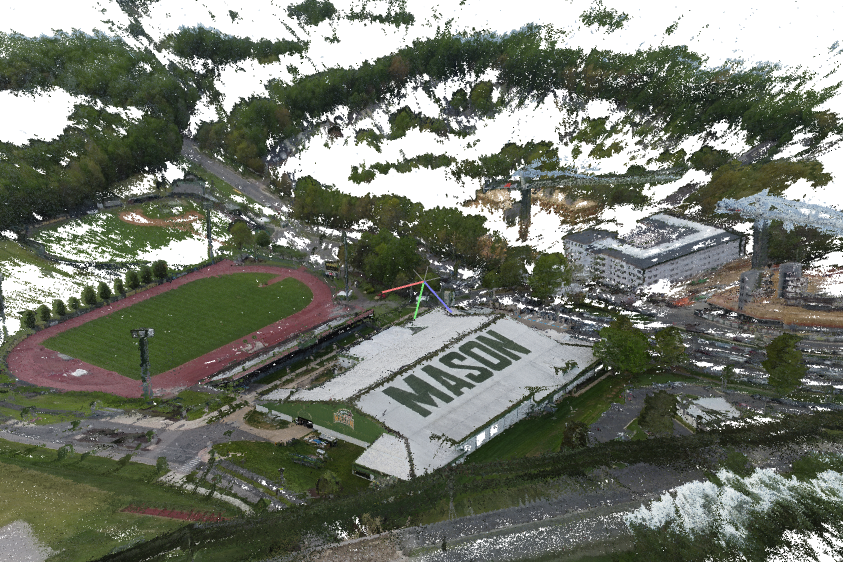
\includegraphics[width=\linewidth,height=6cm,keepaspectratio]{images/results/dense1.png} }}%
    \qquad
    \subfloat[\centering]{{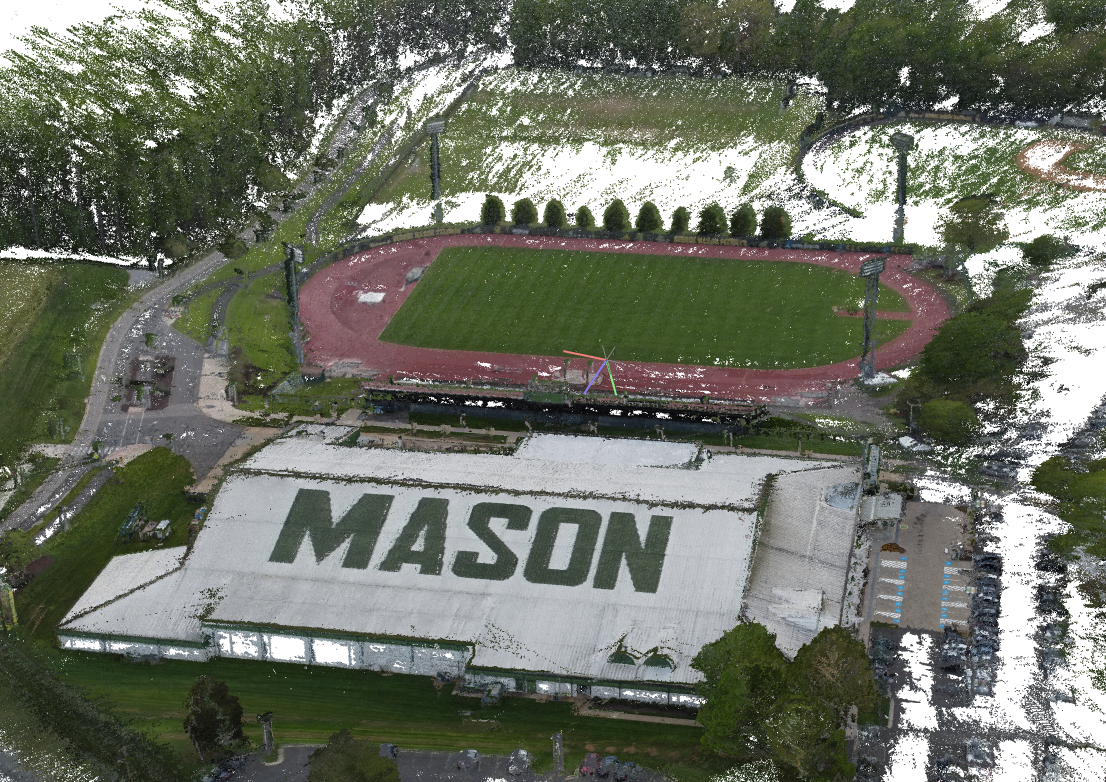
\includegraphics[width=\linewidth]{images/results/dense2.png} }}%
    \qquad
    \subfloat[\centering]{{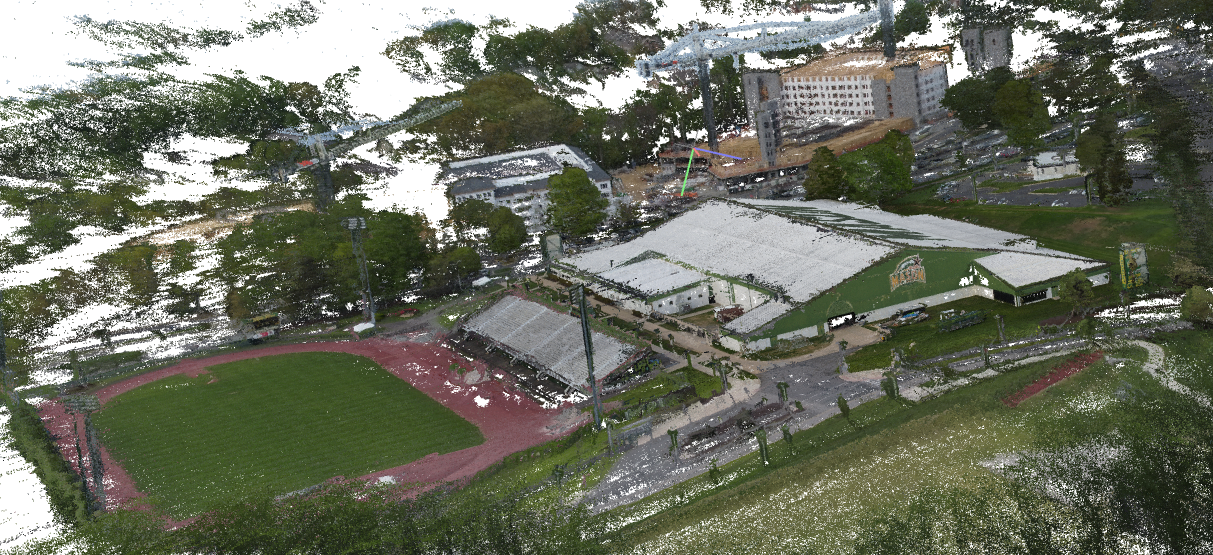
\includegraphics[width=\linewidth]{images/results/dense3.png} }}%
    \caption{Dense Point Cloud of the Reconstruction with 42207561 colored points}
    \label{fig:Dense}%
\end{figure}

\subsection{Latencies Observed While Localizing New Query Images}

 We took 4 Query Images of the Field House and Passed it to REST API for evaluation
\begin{figure}[H]%
    \centering
    \subfloat[\centering 56.4KB]{{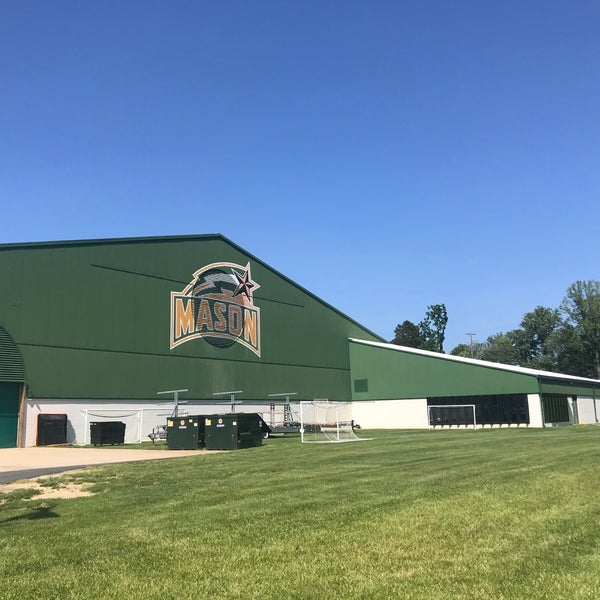
\includegraphics[width=7cm,height=8cm,keepaspectratio]{images/results/query/1.jpg} }}%
    \qquad
    \subfloat[\centering 335.7KB]{{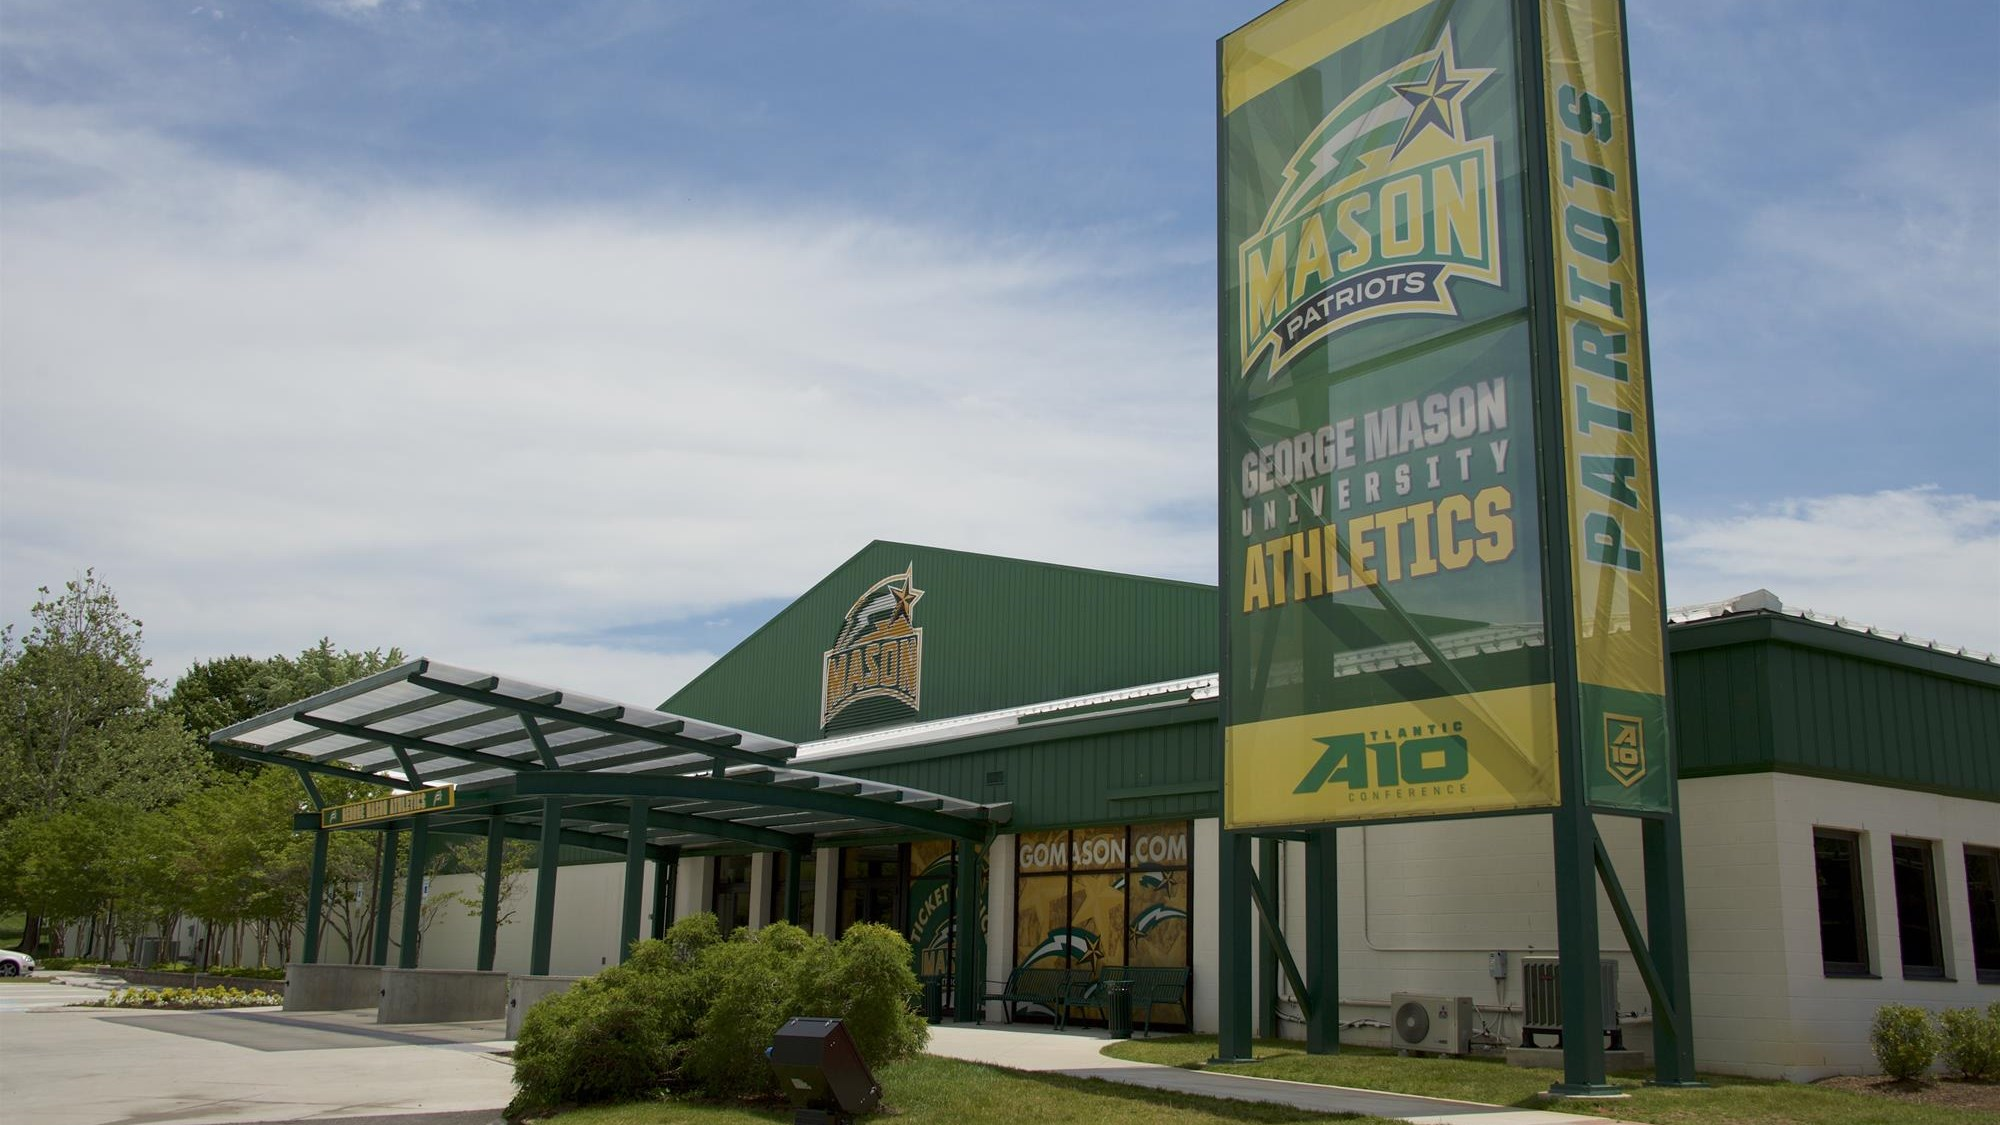
\includegraphics[width=7cm,height=8cm,keepaspectratio]{images/results/query/2.jpg} }}%
    \qquad
    \subfloat[\centering 1.6MB]{{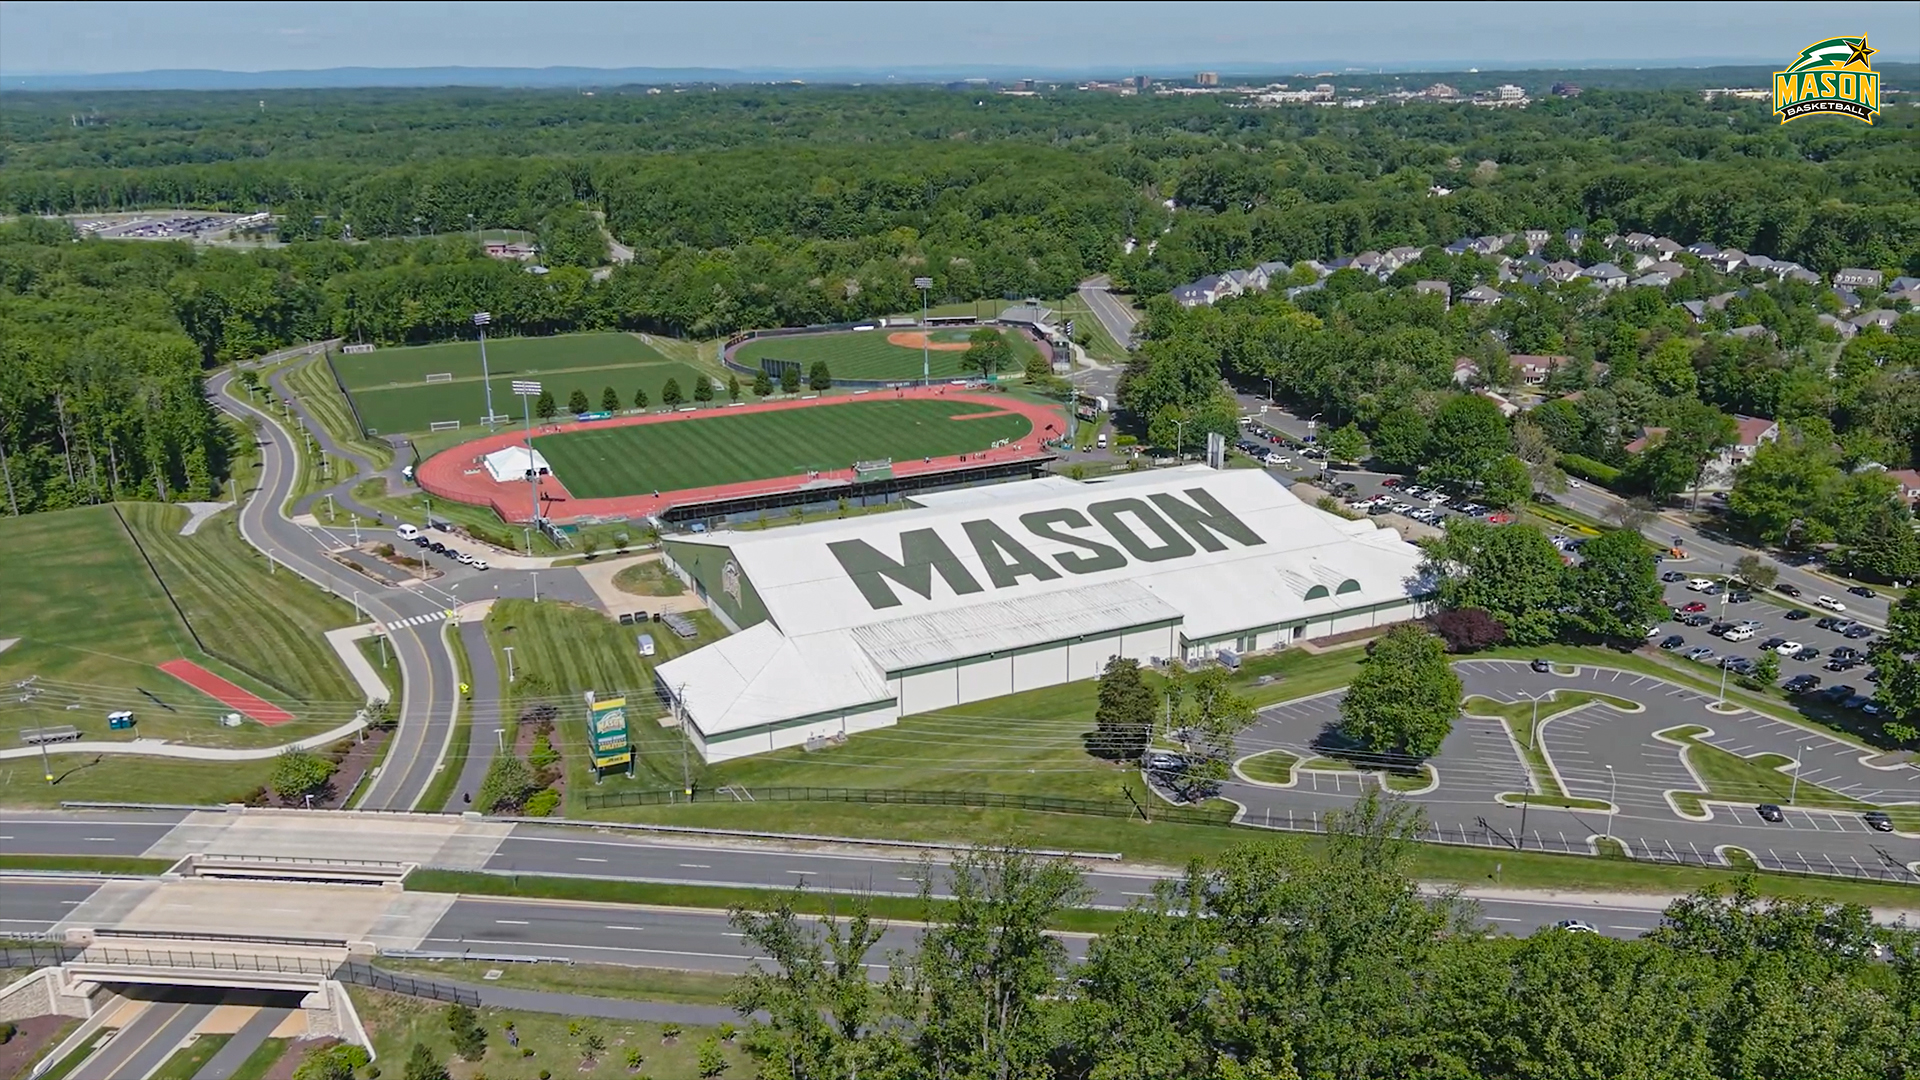
\includegraphics[width=7cm,height=8cm,keepaspectratio]{images/results/query/4.jpg}}}%
    \qquad
    \subfloat[\centering 3.6MB]{{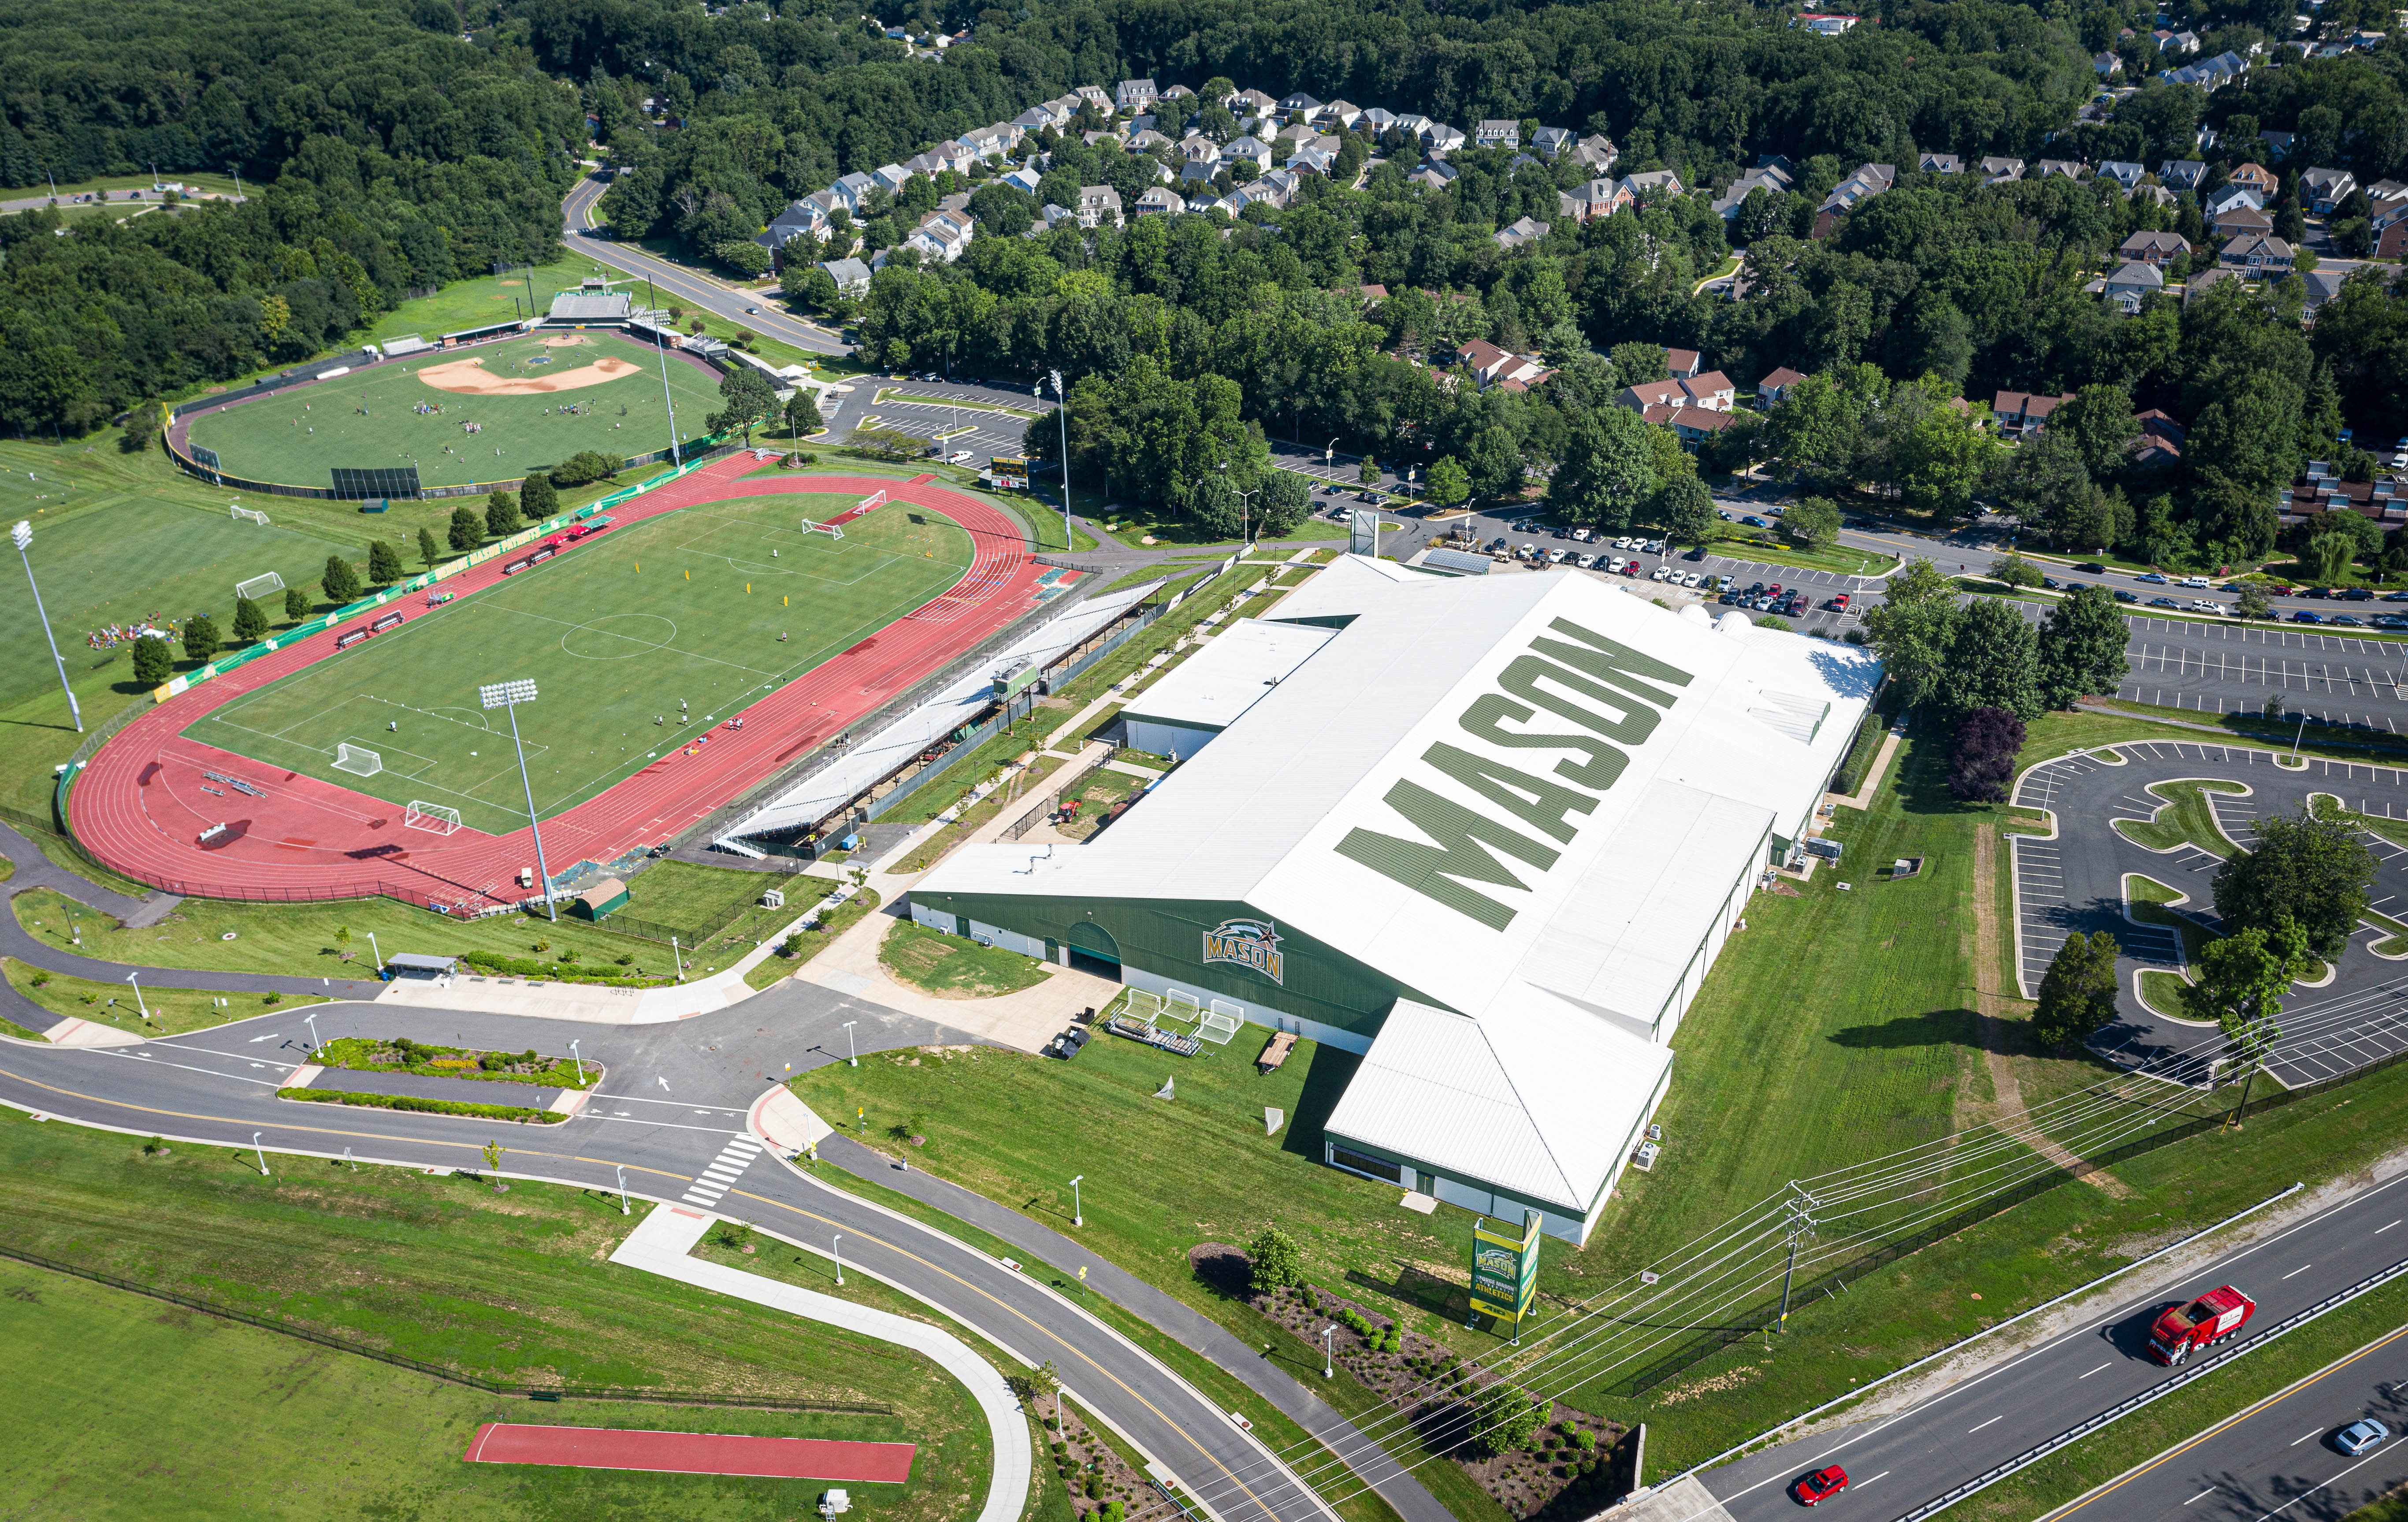
\includegraphics[width=7cm,height=8cm,keepaspectratio]{images/results/query/3.jpg}}}%
    \caption{Query images that were used}
    \label{fig:Query}%
\end{figure}
  

\begin{table}[H]
  \caption{Latencies Observed while Localizing New Query Images}
  \label{tab:latencies}
  \begin{tabular}{cccc}
    \toprule
    Query size & Extractor & Matcher & Latency\\
    \midrule
    56.4 KB & SIFT & NN-Mutual & 15005.703ms\\
    56.4 KB & SuperPoint & SuperGlue & 19587.808ms\\
    335.7 KB & SIFT & NN-Mutual & 12885.49.ms\\
    335.7 KB & SuperPoint & SuperGlue & 27846.842ms\\
    1.6 MB & SIFT & NN-Mutual & 14341.984ms\\
    1.6 MB & SuperPoint & SuperGlue & 30920.418ms\\
    3.6 MB & SIFT & NN-Mutual & 18486.24ms\\
    3.6 MB & SuperPoint & SuperGlue & 48983.89ms\\
  \bottomrule
\end{tabular}
\end{table}

\section{Technical challenges faced}
\begin{itemize}
    \item{As our image dataset was huge, initially we had few issues regarding the computation power as our PC was unable to process and generate a spatial map of the dataset. We solved this problem by running it in an advanced PC with high computational power}
    \item{During the dataset collection, we had to choose a building in George Mason University which doesn't have much glare and other environmental factors such as trees, moving things etc., This process took us multiple attempts and initially, we captured images of Eaglebank Arena and collected the image dataset, but the spatial map generated was incorrect because of the symmetric nature of the arena. Then we moved to capture and collect the dataset of GMU Field house, which we think is one of the best building in George Mason University free of glare and other environmental factors.}
    \item{During performance evaluation, we got few metrics which are incorrect/inaccurate. So, we had to perform the performance evaluation multiple times which were time-consuming}
\end{itemize}

\section{Future work}
\begin{itemize}
    \item{Currently, we are working on calculating the Accuracy of the generated spatial map.}
    \item{We are also developing our mobile application using Unity. Initially, we had less knowledge about the Unity application development, so this took us some time to learn about the framework and start the application development process.}
    \item{After the application is developed, we will integrate our mobile application with the REST API for the localization process.}

We will complete the aforementioned project works before the final project submission deadline.
\end{itemize}

\section{Conclusion}
This research project has focused on evaluating the performance of 6DoF localization on mobile devices, with a particular focus on measuring accuracy and latency. Through our research, we feel that this evaluation plays a crucial role in a variety of applications that require precise and reliable localization, ensuring the practicality and efficiency of these applications.

\section{Acknowledgements}

We thank Dr. Bo Han and Nan Wu from the department of Computer Science at George Mason University. We would also like to thank our classmates and friends for their support and advice given on this research project. Finally, we would like to thank George Mason University for supporting us with available resources.







% \section{Tables}

% The ``\verb|acmart|'' document class includes the ``\verb|booktabs|''
% package --- \url{https://ctan.org/pkg/booktabs} --- for preparing
% high-quality tables.

% Table captions are placed {\itshape above} the table.

% Because tables cannot be split across pages, the best placement for
% them is typically the top of the page nearest their initial cite.  To
% ensure this proper ``floating'' placement of tables, use the
% environment \textbf{table} to enclose the table's contents and the
% table caption.  The contents of the table itself must go in the
% \textbf{tabular} environment, to be aligned properly in rows and
% columns, with the desired horizontal and vertical rules.  Again,
% detailed instructions on \textbf{tabular} material are found in the
% \textit{\LaTeX\ User's Guide}.

% Immediately following this sentence is the point at which
% Table~\ref{tab:freq} is included in the input file; compare the
% placement of the table here with the table in the printed output of
% this document.

% \begin{table}
%   \caption{Frequency of Special Characters}
%   \label{tab:freq}
%   \begin{tabular}{ccl}
%     \toprule
%     Non-English or Math&Frequency&Comments\\
%     \midrule
%     \O & 1 in 1,000& For Swedish names\\
%     $\pi$ & 1 in 5& Common in math\\
%     \$ & 4 in 5 & Used in business\\
%     $\Psi^2_1$ & 1 in 40,000& Unexplained usage\\
%   \bottomrule
% \end{tabular}
% \end{table}

% To set a wider table, which takes up the whole width of the page's
% live area, use the environment \textbf{table*} to enclose the table's
% contents and the table caption.  As with a single-column table, this
% wide table will ``float'' to a location deemed more
% desirable. Immediately following this sentence is the point at which
% Table~\ref{tab:commands} is included in the input file; again, it is
% instructive to compare the placement of the table here with the table
% in the printed output of this document.

% \begin{table*}
%   \caption{Some Typical Commands}
%   \label{tab:commands}
%   \begin{tabular}{ccl}
%     \toprule
%     Command &A Number & Comments\\
%     \midrule
%     \texttt{{\char'134}author} & 100& Author \\
%     \texttt{{\char'134}table}& 300 & For tables\\
%     \texttt{{\char'134}table*}& 400& For wider tables\\
%     \bottomrule
%   \end{tabular}
% \end{table*}

% Always use midrule to separate table header rows from data rows, and
% use it only for this purpose. This enables assistive technologies to
% recognise table headers and support their users in navigating tables
% more easily.

% \section{Math Equations}
% You may want to display math equations in three distinct styles:
% inline, numbered or non-numbered display.  Each of the three are
% discussed in the next sections.

% \subsection{Inline (In-text) Equations}
% A formula that appears in the running text is called an inline or
% in-text formula.  It is produced by the \textbf{math} environment,
% which can be invoked with the usual
% \texttt{{\char'134}begin\,\ldots{\char'134}end} construction or with
% the short form \texttt{\$\,\ldots\$}. You can use any of the symbols
% and structures, from $\alpha$ to $\omega$, available in
% \LaTeX~\cite{Lamport:LaTeX}; this section will simply show a few
% examples of in-text equations in context. Notice how this equation:
% \begin{math}
%   \lim_{n\rightarrow \infty}x=0
% \end{math},
% set here in in-line math style, looks slightly different when
% set in display style.  (See next section).

% \subsection{Display Equations}
% A numbered display equation---one set off by vertical space from the
% text and centered horizontally---is produced by the \textbf{equation}
% environment. An unnumbered display equation is produced by the
% \textbf{displaymath} environment.

% Again, in either environment, you can use any of the symbols and
% structures available in \LaTeX\@; this section will just give a couple
% of examples of display equations in context.  First, consider the
% equation, shown as an inline equation above:
% \begin{equation}
%   \lim_{n\rightarrow \infty}x=0
% \end{equation}
% Notice how it is formatted somewhat differently in
% the \textbf{displaymath}
% environment.  Now, we'll enter an unnumbered equation:
% \begin{displaymath}
%   \sum_{i=0}^{\infty} x + 1
% \end{displaymath}
% and follow it with another numbered equation:
% \begin{equation}
%   \sum_{i=0}^{\infty}x_i=\int_{0}^{\pi+2} f
% \end{equation}
% just to demonstrate \LaTeX's able handling of numbering.

% \section{Figures}

% The ``\verb|figure|'' environment should be used for figures. One or
% more images can be placed within a figure. If your figure contains
% third-party material, you must clearly identify it as such, as shown
% in the example below.
% \begin{figure}[h]
%   \centering
%   \includegraphics[width=\linewidth]{sample-franklin}
%   \caption{1907 Franklin Model D roadster. Photograph by Harris \&
%     Ewing, Inc. [Public domain], via Wikimedia
%     Commons. (\url{https://goo.gl/VLCRBB}).}
%   \Description{A woman and a girl in white dresses sit in an open car.}
% \end{figure}

% Your figures should contain a caption which describes the figure to
% the reader.

% Figure captions are placed {\itshape below} the figure.

% Every figure should also have a figure description unless it is purely
% decorative. These descriptions convey what’s in the image to someone
% who cannot see it. They are also used by search engine crawlers for
% indexing images, and when images cannot be loaded.

% A figure description must be unformatted plain text less than 2000
% characters long (including spaces).  {\bfseries Figure descriptions
%   should not repeat the figure caption – their purpose is to capture
%   important information that is not already provided in the caption or
%   the main text of the paper.} For figures that convey important and
% complex new information, a short text description may not be
% adequate. More complex alternative descriptions can be placed in an
% appendix and referenced in a short figure description. For example,
% provide a data table capturing the information in a bar chart, or a
% structured list representing a graph.  For additional information
% regarding how best to write figure descriptions and why doing this is
% so important, please see
% \url{https://www.acm.org/publications/taps/describing-figures/}.

% \subsection{The ``Teaser Figure''}

% A ``teaser figure'' is an image, or set of images in one figure, that
% are placed after all author and affiliation information, and before
% the body of the article, spanning the page. If you wish to have such a
% figure in your article, place the command immediately before the
% \verb|\maketitle| command:
% \begin{verbatim}
%   \begin{teaserfigure}
%     \includegraphics[width=\textwidth]{sampleteaser}
%     \caption{figure caption}
%     \Description{figure description}
%   \end{teaserfigure}
% \end{verbatim}

% \section{Citations and Bibliographies}

% The use of \BibTeX\ for the preparation and formatting of one's
% references is strongly recommended. Authors' names should be complete
% --- use full first names (``Donald E. Knuth'') not initials
% (``D. E. Knuth'') --- and the salient identifying features of a
% reference should be included: title, year, volume, number, pages,
% article DOI, etc.

% The bibliography is included in your source document with these two
% commands, placed just before the \verb|\end{document}| command:
% \begin{verbatim}
%   \bibliographystyle{ACM-Reference-Format}
%   \bibliography{bibfile}
% \end{verbatim}
% where ``\verb|bibfile|'' is the name, without the ``\verb|.bib|''
% suffix, of the \BibTeX\ file.

% Citations and references are numbered by default. A small number of
% ACM publications have citations and references formatted in the
% ``author year'' style; for these exceptions, please include this
% command in the {\bfseries preamble} (before the command
% ``\verb|\begin{document}|'') of your \LaTeX\ source:
% \begin{verbatim}
%   \citestyle{acmauthoryear}
% \end{verbatim}


%   Some examples.  A paginated journal article \cite{Abril07}, an
%   enumerated journal article \cite{Cohen07}, a reference to an entire
%   issue \cite{JCohen96}, a monograph (whole book) \cite{Kosiur01}, a
%   monograph/whole book in a series (see 2a in spec. document)
%   \cite{Harel79}, a divisible-book such as an anthology or compilation
%   \cite{Editor00} followed by the same example, however we only output
%   the series if the volume number is given \cite{Editor00a} (so
%   Editor00a's series should NOT be present since it has no vol. no.),
%   a chapter in a divisible book \cite{Spector90}, a chapter in a
%   divisible book in a series \cite{Douglass98}, a multi-volume work as
%   book \cite{Knuth97}, a couple of articles in a proceedings (of a
%   conference, symposium, workshop for example) (paginated proceedings
%   article) \cite{Andler79, Hagerup1993}, a proceedings article with
%   all possible elements \cite{Smith10}, an example of an enumerated
%   proceedings article \cite{VanGundy07}, an informally published work
%   \cite{Harel78}, a couple of preprints \cite{Bornmann2019,
%     AnzarootPBM14}, a doctoral dissertation \cite{Clarkson85}, a
%   master's thesis: \cite{anisi03}, an online document / world wide web
%   resource \cite{Thornburg01, Ablamowicz07, Poker06}, a video game
%   (Case 1) \cite{Obama08} and (Case 2) \cite{Novak03} and \cite{Lee05}
%   and (Case 3) a patent \cite{JoeScientist001}, work accepted for
%   publication \cite{rous08}, 'YYYYb'-test for prolific author
%   \cite{SaeediMEJ10} and \cite{SaeediJETC10}. Other cites might
%   contain 'duplicate' DOI and URLs (some SIAM articles)
%   \cite{Kirschmer:2010:AEI:1958016.1958018}. Boris / Barbara Beeton:
%   multi-volume works as books \cite{MR781536} and \cite{MR781537}. A
%   couple of citations with DOIs:
%   \cite{2004:ITE:1009386.1010128,Kirschmer:2010:AEI:1958016.1958018}. Online
%   citations: \cite{TUGInstmem, Thornburg01, CTANacmart}.
%   Artifacts: \cite{R} and \cite{UMassCitations}.

% \section{Acknowledgments}

% Identification of funding sources and other support, and thanks to
% individuals and groups that assisted in the research and the
% preparation of the work should be included in an acknowledgment
% section, which is placed just before the reference section in your
% document.

% This section has a special environment:
% \begin{verbatim}
%   \begin{acks}
%   ...
%   \end{acks}
% \end{verbatim}
% so that the information contained therein can be more easily collected
% during the article metadata extraction phase, and to ensure
% consistency in the spelling of the section heading.

% Authors should not prepare this section as a numbered or unnumbered {\verb|\section|}; please use the ``{\verb|acks|}'' environment.

% \section{Appendices}

% If your work needs an appendix, add it before the
% ``\verb|\end{document}|'' command at the conclusion of your source
% document.

% Start the appendix with the ``\verb|appendix|'' command:
% \begin{verbatim}
%   \appendix
% \end{verbatim}
% and note that in the appendix, sections are lettered, not
% numbered. This document has two appendices, demonstrating the section
% and subsection identification method.

% \section{Multi-language papers}

% Papers may be written in languages other than English or include
% titles, subtitles, keywords and abstracts in different languages (as a
% rule, a paper in a language other than English should include an
% English title and an English abstract).  Use \verb|language=...| for
% every language used in the paper.  The last language indicated is the
% main language of the paper.  For example, a French paper with
% additional titles and abstracts in English and German may start with
% the following command
% \begin{verbatim}
% \documentclass[sigconf, language=english, language=german,
%                language=french]{acmart}
% \end{verbatim}

% The title, subtitle, keywords and abstract will be typeset in the main
% language of the paper.  The commands \verb|\translatedXXX|, \verb|XXX|
% begin title, subtitle and keywords, can be used to set these elements
% in the other languages.  The environment \verb|translatedabstract| is
% used to set the translation of the abstract.  These commands and
% environment have a mandatory first argument: the language of the
% second argument.  See \verb|sample-sigconf-i13n.tex| file for examples
% of their usage.

% \section{SIGCHI Extended Abstracts}

% The ``\verb|sigchi-a|'' template style (available only in \LaTeX\ and
% not in Word) produces a landscape-orientation formatted article, with
% a wide left margin. Three environments are available for use with the
% ``\verb|sigchi-a|'' template style, and produce formatted output in
% the margin:
% \begin{description}
% \item[\texttt{sidebar}:]  Place formatted text in the margin.
% \item[\texttt{marginfigure}:] Place a figure in the margin.
% \item[\texttt{margintable}:] Place a table in the margin.
% \end{description}

% %%
% %% The acknowledgments section is defined using the "acks" environment
% %% (and NOT an unnumbered section). This ensures the proper
% %% identification of the section in the article metadata, and the
% %% consistent spelling of the heading.
% \begin{acks}
% To Robert, for the bagels and explaining CMYK and color spaces.
% \end{acks}

%%
%% The next two lines define the bibliography style to be used, and
%% the bibliography file.
\bibliographystyle{ACM-Reference-Format}
\bibliography{bibliography.bib}


%%
%% If your work has an appendix, this is the place to put it.
% \appendix

% \section{Research Methods}

% \subsection{Part One}

% Lorem ipsum dolor sit amet, consectetur adipiscing elit. Morbi
% malesuada, quam in pulvinar varius, metus nunc fermentum urna, id
% sollicitudin purus odio sit amet enim. Aliquam ullamcorper eu ipsum
% vel mollis. Curabitur quis dictum nisl. Phasellus vel semper risus, et
% lacinia dolor. Integer ultricies commodo sem nec semper.

% \subsection{Part Two}

% Etiam commodo feugiat nisl pulvinar pellentesque. Etiam auctor sodales
% ligula, non varius nibh pulvinar semper. Suspendisse nec lectus non
% ipsum convallis congue hendrerit vitae sapien. Donec at laoreet
% eros. Vivamus non purus placerat, scelerisque diam eu, cursus
% ante. Etiam aliquam tortor auctor efficitur mattis.

% \section{Online Resources}

% Nam id fermentum dui. Suspendisse sagittis tortor a nulla mollis, in
% pulvinar ex pretium. Sed interdum orci quis metus euismod, et sagittis
% enim maximus. Vestibulum gravida massa ut felis suscipit
% congue. Quisque mattis elit a risus ultrices commodo venenatis eget
% dui. Etiam sagittis eleifend elementum.

% Nam interdum magna at lectus dignissim, ac dignissim lorem
% rhoncus. Maecenas eu arcu ac neque placerat aliquam. Nunc pulvinar
% massa et mattis lacinia.

\end{document}
\endinput
%%
%% End of file `sample-sigconf.tex'.